
%% For double-blind review submission, w/o CCS and ACM Reference (max submission space)
\documentclass[sigplan,10pt, review,anonymous]{acmart}
%\documentclass[sigplan,screen]{acmart} 
\settopmatter{printfolios=false,printccs=false,printacmref=false}
%\settopmatter{printacmref=false, printfolios=false}
%% For double-blind review submission, w/ CCS and ACM Reference
%\documentclass[sigplan,review,anonymous]{acmart}\settopmatter{printfolios=true}
%% For single-blind review submission, w/o CCS and ACM Reference (max submission space)
%\documentclass[sigplan,review]{acmart}\settopmatter{printfolios=true,printccs=false,printacmref=false}
%% For single-blind review submission, w/ CCS and ACM Reference
%\documentclass[sigplan,review]{acmart}\settopmatter{printfolios=true}
%% For final camera-ready submission, w/ required CCS and ACM Reference
%\documentclass[sigplan]{acmart}\settopmatter{}


%%
%% This is file `sample-sigconf.tex',
%% generated with the docstrip utility.
%%
%% The original source files were:
%%
%% samples.dtx  (with options: `sigconf')
%% 
%% IMPORTANT NOTICE:
%% 
%% For the copyright see the source file.
%% 
%% Any modified versions of this file must be renamed
%% with new filenames distinct from sample-sigconf.tex.
%% 
%% For distribution of the original source see the terms
%% for copying and modification in the file samples.dtx.
%% 
%% This generated file may be distributed as long as the
%% original source files, as listed above, are part of the
%% same distribution. (The sources need not necessarily be
%% in the same archive or directory.)
%%
%% Commands for TeXCount
%TC:macro \cite [option:text,text]
%TC:macro \citep [option:text,text]
%TC:macro \citet [option:text,text]
%TC:envir table 0 1
%TC:envir table* 0 1
%TC:envir tabular [ignore] word
%TC:envir displaymath 0 word
%TC:envir math 0 word
%TC:envir comment 0 0
%%
%%
%% The first command in your LaTeX source must be the \documentclass command.
%\documentclass[sigconf]{acmart}

\usepackage[english]{babel}
\usepackage{blindtext}
\usepackage{multirow}
\usepackage{CJKutf8}

\usepackage{booktabs}
\usepackage{subfigure}
\usepackage{xspace}
%%\usepackage{amsmath}
\usepackage{epstopdf} 
\usepackage{algorithm}
\usepackage{url}
%%\usepackage{algorithmicx} 
\usepackage{algpseudocode}
%%\usepackage{color}
\usepackage{ulem}

\newcommand{\btree} {B+tree\xspace}
\newcommand{\txtree}{STM-based GPU \btree\xspace}
\newcommand{\base}{STM-based GPU B+tree\xspace}
\newcommand{\baseshort}{STM GB-tree\xspace}
\newcommand{\locktree}{lock-baed GB-tree\xspace}
\newcommand{\ucdavis}{lock-based GPU B-tree\xspace}
\newcommand{\ucdavisshort}{Lock GB-tree\xspace}
\newcommand{\sys} {uniRDMA\xspace}
\newcommand{\native} {bare-metal RDMA\xspace}

%% NOTE that a single column version may be required for 
%% submission and peer review. This can be done by changing
%% the \doucmentclass[...]{acmart} in this template to 
%% \documentclass[manuscript,screen]{acmart}
%% 
%% To ensure 100% compatibility, please check the white list of
%% approved LaTeX packages to be used with the Master Article Template at
%% https://www.acm.org/publications/taps/whitelist-of-latex-packages 
%% before creating your document. The white list page provides 
%% information on how to submit additional LaTeX packages for 
%% review and adoption.
%% Fonts used in the template cannot be substituted; margin 
%% adjustments are not allowed.
%%
%%
%% \BibTeX command to typeset BibTeX logo in the docs
\AtBeginDocument{%
  \providecommand\BibTeX{{%
    \normalfont B\kern-0.5em{\scshape i\kern-0.25em b}\kern-0.8em\TeX}}}

%% Rights management information.  This information is sent to you
%% when you complete the rights form.  These commands have SAMPLE
%% values in them; it is your responsibility as an author to replace
%% the commands and values with those provided to you when you
%% complete the rights form.
%\setcopyright{acmcopyright}
%\copyrightyear{2018}
%\acmYear{2018}
%\acmDOI{XXXXXXX.XXXXXXX}



%%% These commands are for a PROCEEDINGS abstract or paper.
%\acmConference[Conference acronym 'XX]{Make sure to enter the correct
%  conference title from your rights confirmation emai}{June 03--05,
%  2018}{Woodstock, NY}
%%
%%  Uncomment \acmBooktitle if th title of the proceedings is different
%%  from ``Proceedings of ...''!
%%
%%\acmBooktitle{Woodstock '18: ACM Symposium on Neural Gaze Detection,
%%  June 03--05, 2018, Woodstock, NY} 
%\acmPrice{15.00}
%\acmISBN{978-1-4503-XXXX-X/18/06}


%%
%% Submission ID.
%% Use this when submitting an article to a sponsored event. You'll
%% receive a unique submission ID from the organizers
%% of the event, and this ID should be used as the parameter to this command.
%%\acmSubmissionID{123-A56-BU3}

%%
%% For managing citations, it is recommended to use bibliography
%% files in BibTeX format.
%%
%% You can then either use BibTeX with the ACM-Reference-Format style,
%% or BibLaTeX with the acmnumeric or acmauthoryear sytles, that include
%% support for advanced citation of software artefact from the
%% biblatex-software package, also separately available on CTAN.
%%
%% Look at the sample-*-biblatex.tex files for templates showcasing
%% the biblatex styles.
%%

%%
%% The majority of ACM publications use numbered citations and
%% references.  The command \citestyle{authoryear} switches to the
%% "author year" style.
%%
%% If you are preparing content for an event
%% sponsored by ACM SIGGRAPH, you must use the "author year" style of
%% citations and references.
%% Uncommenting
%% the next command will enable that style.
%%\citestyle{acmauthoryear}

%%
%% end of the preamble, start of the body of the document source.
\begin{document}

%%
%% The "title" command has an optional parameter,
%% allowing the author to define a "short title" to be used in page headers.
\title{\sys: Unified Virtual RDMA for Hybrid Virtual Environments}


%\author{Anonymous authors}
%\affiliation{%
%	\institution{Paper under double-blind review}
%	\city{}
%	\country{}
%}
%\email{}
%%
%% The "author" command and its associated commands are used to define
%% the authors and their affiliations.
%% Of note is the shared affiliation of the first two authors, and the
%% "authornote" and "authornotemark" commands
%% used to denote shared contribution to the research.


%%
%% By default, the full list of authors will be used in the page
%% headers. Often, this list is too long, and will overlap
%% other information printed in the page headers. This command allows
%% the author to define a more concise list
%% of authors' names for this purpose.
%-----------------\renewcommand{\shortauthors}{Anonymous Author, et al.}




%%
%% The abstract is a short summary of the work to be presented in the
%% article.

\begin{abstract}
Supercomputing is important in most data-driven fileds for its extrem high-performance, such as such as artificial intelligence and large-scale data processing. As the developement of cloud, supercomputing is also in virtual machines or containers for effiecncy and elasticity. Today, hybrid virtual enviroments is a trend in most datacenters because of combined advatanges and historic reasons. RDMA is neccesay in supercomputing for its high network performance. However, existing RDMA virtualization solutions lack centralized virtualization layer and general interfaces for hybrid virtual environments. To solve this problem, we present uniRDMA, a generic RDMA software virtualization framework that consists of single virtual layer and general uniVerbs interfaces. The centralized user space virtual layer constructs multiple isolated vRNICs(virtual RDMA NICs) with the help of hardware virtualization technology and realizes a unified virtual RDMA network. To realize both generality and high-performance, uniVerbs interfaces use shared memory as I/O approach for RDMA applications and map RDMA resources to vRNIC. In our evaluation based on uniRDMA prototype, the performance and scalability of uniRDMA is close to bare-metal RDMA in virtual machines, containers and hybrid cloud environments.
\end{abstract}


%%
%% The code below is generated by the tool at http://dl.acm.org/ccs.cfm.
%% Please copy and paste the code instead of the example below.
%%
%\begin{CCSXML}
%<ccs2012>
% <concept>
%  <concept_id>10010520.10010553.10010562</concept_id>
%  <concept_desc>Computer systems organization~Embedded systems</concept_desc>
%  <concept_significance>500</concept_significance>
% </concept>
% <concept>
%  <concept_id>10010520.10010575.10010755</concept_id>
%  <concept_desc>Computer systems organization~Redundancy</concept_desc>
%  <concept_significance>300</concept_significance>
% </concept>
% <concept>
%  <concept_id>10010520.10010553.10010554</concept_id>
%  <concept_desc>Computer systems organization~Robotics</concept_desc>
%  <concept_significance>100</concept_significance>
% </concept>
% <concept>
%  <concept_id>10003033.10003083.10003095</concept_id>
%  <concept_desc>Networks~Network reliability</concept_desc>
%  <concept_significance>100</concept_significance>
% </concept>
%</ccs2012>
%\end{CCSXML}
%
%\ccsdesc[500]{Computer systems organization~Embedded systems}
%\ccsdesc[300]{Computer systems organization~Redundancy}
%\ccsdesc{Computer systems organization~Robotics}
%\ccsdesc[100]{Networks~Network reliability}

%%
%% Keywords. The author(s) should pick words that accurately describe
%% the work being presented. Separate the keywords with commas.
\keywords{RDMA, virtualization, virtual machine, contianer}

%% A "teaser" image appears between the author and affiliation
%% information and the body of the document, and typically spans the
%% page.

%%
%% This command processes the author and affiliation and title
%% information and builds the first part of the formatted document.


\maketitle




\section{Introduction}
RDMA(remote direct memory access), is a new type of high-performance network technology. RDMA is currently widely used in artificial intelligence, data processing, and high-performance computing. For examples, TensorFlow, Spark, and Hadoop [21] all have supported RDMA. With hardware protocol stack and zero copy technologies, RNICs(physical RDMA network cards) can bypass the kernel to read/write remote memory data according to the work requests of applications, without the participation of remote CPU. Therefore, RDMA has high throughput, low latency and low CPU load.

The core technology of cloud computing is virtualization, mainly including container and virtual machine. The container is a lightweight isolated runtime environment, does not need device emulation, and has low performance loss. The virtual machine has strong isolation and is more secure, but the performance loss is large. Both virtual machines and containers have been widely used, and the trend has become the unified deployment and management for hybrid virtual environments. For example, VMware's virtualization platform vSphere and ReadHat's container cloud platform OpenShift, both clearly support the unified deployment and management of virtual machines and containers in the latest version.

RDMA virtualization is necessary for cloud applications to exploit RDMA. RDMA virtualization not only needs to maintain high performance and manageability, but also have generality for hybrid virtual environments. Therefore, our RDMA virtualization goals are as follows:

\begin{itemize}
\item {\verb|Generality|}: To form unified RDMA virtualization, single centralized virtual layer should be set up, which is provided to virtual machines and containers with general interfaces.
\item {\verb|High performance|}: Virtual RDMA should be close to native RDMA in terms of throughput, latency, and CPU load. Meanwhile it should be suit for large-scale virtual cluster.
\item {\verb|High manageability|}: In RDMA virtualization, container and virtual machine characteristics should be maintained to realize portability, isolation and network management.
\end{itemize}

RDMA has different hardware characteristics and working mechanisms compared to traditional network. Therefore, RDMA virtualization is different from traditional network virtualization. Current RDMA virtualization work mainly includes hardware virtualization and software virtualization. However, none of the existing solutions can meet all above goals.

The representative of hardware virtualization is SR-IOV. Its virtual layer is located in the hardware. Although the isolation and high performance are maintained,  SR-IOV lacks portability and other manageability without software virtual layer. In software virtualization, existing solutions treat virtual machines and containers differently. For containers, FreeFlowl~\cite{kim2019freeflow} forwards all RDMA commands to the virtual layer, and that is ineffective because of losing RDMA's kernel by-pass. For virtual machines, HyV avoids forwarding overhead by mapping RDMA resources, but lacks the management of virtual RDMA networks; although MasQ makes up for this problem, its virtual layer is located in kernel space. Extending MasQ to the container environment will lose lightweight  management in user space for containers.

We proposes an unified RDMA virtualization framework for both containers and virtual machines, namely uniRDMA, which achieves high performance and high manageability. UniRDMA is mainly composed of single centralized uniRDMA virtual layer and general uniVerbs interfaces. All managements are concentrated in the user space virtual layer; the UniVerbs interface is general to the RDMA applications in virtual machines or containers.

There are mainly two challenges in the design of uniRDMA: First, virtual machines and containers are essentially different virtualization technologies. Virtual machines are under the management of hypervisor in kernel space, containers are isolted runtime mainly about user space. It is a challenge to build a centralized virtual layer for both containers and virtual machines; second, mapping all RDMA resources is the key idea to achive high performance. However, the existing solutions only implement the mapping operation in the same process for virtual machine. In this paper, the virtual layer belongs to another host process. So, it is also another challenge to map all RDMA resources.

To address the first challenge, uniRDMA separates the control and use of RDMA resources in virtulization, builds multiple vRNICs in single unified user space virtualization layer. Each vRNIC encapsulates virtual RDMA resources, and isolates with others by hardware virtualization. Moreover, through a common file-based shared memory queue, each vRNIC has a general interface for virtual machines and containers. For the second challenge,  at first, virtual RDMA resources in vRNICs are mapped to physical RNICs, and then shared memory are used to ensure RDMA resources in applications are mapped to vRNICs in the virtual layer.

We implements the prototype of uniRDMA and evaluate uniRDMA against with hardware virtualization, software virtualization FreeFlow, and native RDMA in different benchmarks, such as throughput, latency, scalability, and real-word applications. From the result, uniRDMA's performance is close to native RDMA in both virtual machine and container environments, and is significantly better than FreeFlow. The throughput can reach up to 6 times that of FreeFlow, and the latency can reach down to 40\% of FreeFlow.uniRDMA also has high scalability and adapts to real-world RDMA applications in hybrid cloud environments.

The main contributions in this paper are as follows:

(1)Unified RDMA virtulization in hybrid virtual environments is firstly proposed in this paper and uniRDMA is general RDMA virtualization framework,  while maintaining high performance and high manageability.

(2)uniRDMA are evaluated and the results proved that uniRDMA maintains high performance close to native RDMA.


\section{RDMA Background} \label{background}
RDMA infrastructure is built for distributed applications that require high-performance and low latency network communications. It uses a zero copy approach to deliver data between servers. With RDMA, applications can read and write memory of a remote machine, without the participation of CPU and OS kernel on both sides.

\begin{figure}[!ht]
	\centering
	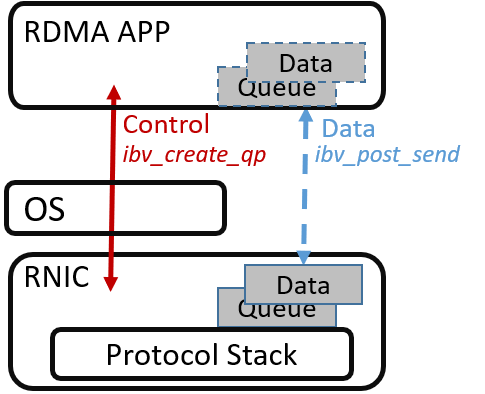
\includegraphics[width=0.8\linewidth]{images/rdma-feat.png}
	\caption{Native RDMA Architecture: the control path and data path are separated}
	\label{fig:rdma-feat}
\end{figure}

RDMA can be implemented in different ways, for example, InfiniBand~\cite{infiniband}, Roce~\cite{roce}, and iWARP~\cite{iwarp}.
OpenFabrics Enterprise Distribution (OFED \cite{ofed}) is a widely used RDMA software stack that builds an abstraction layer to hide the differences of underneath drivers and hardware.
OFED stack consists of the user-space part and the kernel-space part.
As shown in Figure~\ref{fig:rdma-feat}, in user-space, RDMA applications use Verbs APIs~\cite{verbs} to send and receive data. It is similar to socket layer for traditional network applications. On the control path, Verbs provides APIs like ibv\_create\_qp and ibv\_reg\_mr. On the data path, Verbs provides APIs like ibv\_post\_send and ibv\_post\_recv. On the control path, the Verbs library forwards requests to OFED core in OS kernel. Device specific drivers that control the RDMA hardware are registered in OFED core. On the data path, the OS kernel is bypassed. So the Verbs library calls device specific user level library to send and receive data.

In the workflow of RDMA, the control path and the data path are separated. As shown in Figure~\ref{fig:rdma-feat}, on the control path, the application explicitly creates QP~(Queue Pair), CQ~(Completed Queue), registers MR~(Memory Region) and other RDMA metadata, and caches the metadata to RNIC, such as queue ID, MR key and page tables. On the data path, the application can write to the DoorBell register to notify RNIC of a new request. RNIC will read the request in the QP, read/write the contents of the local/remote MR, and put the completion notifications into the CQ. The application can poll the CQ to get the notifications. The housekeeping work is done on the control path that involves the OS kernel. The performance critical data transmission work on the data path totally bypasses the OS kernel.
%%\section{Overview}
The architecture of uniRDMA is shown in Figure~\ref{fig:framework-overview}. uniRDMA mainly consists of vRNIC, which is a para-virtualization device for guest, and the management layer(虚拟层暂定为管理层). Besides, some modifications are made to RDMA user library and device specific drivers for cooperating with uniRDMA.

(1) vRNIC frontend and backend: vRNIC frontend is as the device driver of hosts' backend. It cooperates with modified verbs and device-specific libraries and forwards serial commands to backend. In specific, the frontend is in kernel for VMs. vRNIC backend is as virtual device in host user space. It execute received commands. To achieve high performance, the control path and data path are separate in vRNICs. For data path, vRNIC frontend does not forwards RDMA commands, and directly use the mapped RDMA resources (e.g. QPs or MRs). The resources are mapped to backend by shared memory.

(2) Management Layer: To make a centralized management, a management center connect with each host's uniRDMA backend. The management mainly includes vRNIC device management and network management. For device management, the layer coordinates the hardware resources (e.g. VFs in SR-IOV) to achieve the hardware-support functions effectively, e.g. performance isolation. For network management, the layer can construct a virtual RDMA network by software methods, including configuring each vRNIC address, defining routing rules and maintaining the mapping for vRNIC connections. (包含设备管理和网络管理两个部分,设备管理主要是协调硬件虚拟化VF资源,网络管理是纯软件实现,包括配置vRNIC地址和路由规则等)

Besides, to support transparency for applications in guest, we modified the verbs library and hardware-specific libraries in guest. After modification, the RDMA commands can be forwarded to vRNIC frontends. Also, the memory of RDMA resources (e.g. QPs) can be backend with our shared memory. (必须修改设备相关库,RDMA QP资源的内存才能够用我们的共享内存去支持)

\begin{figure}[!ht]
	\centering
	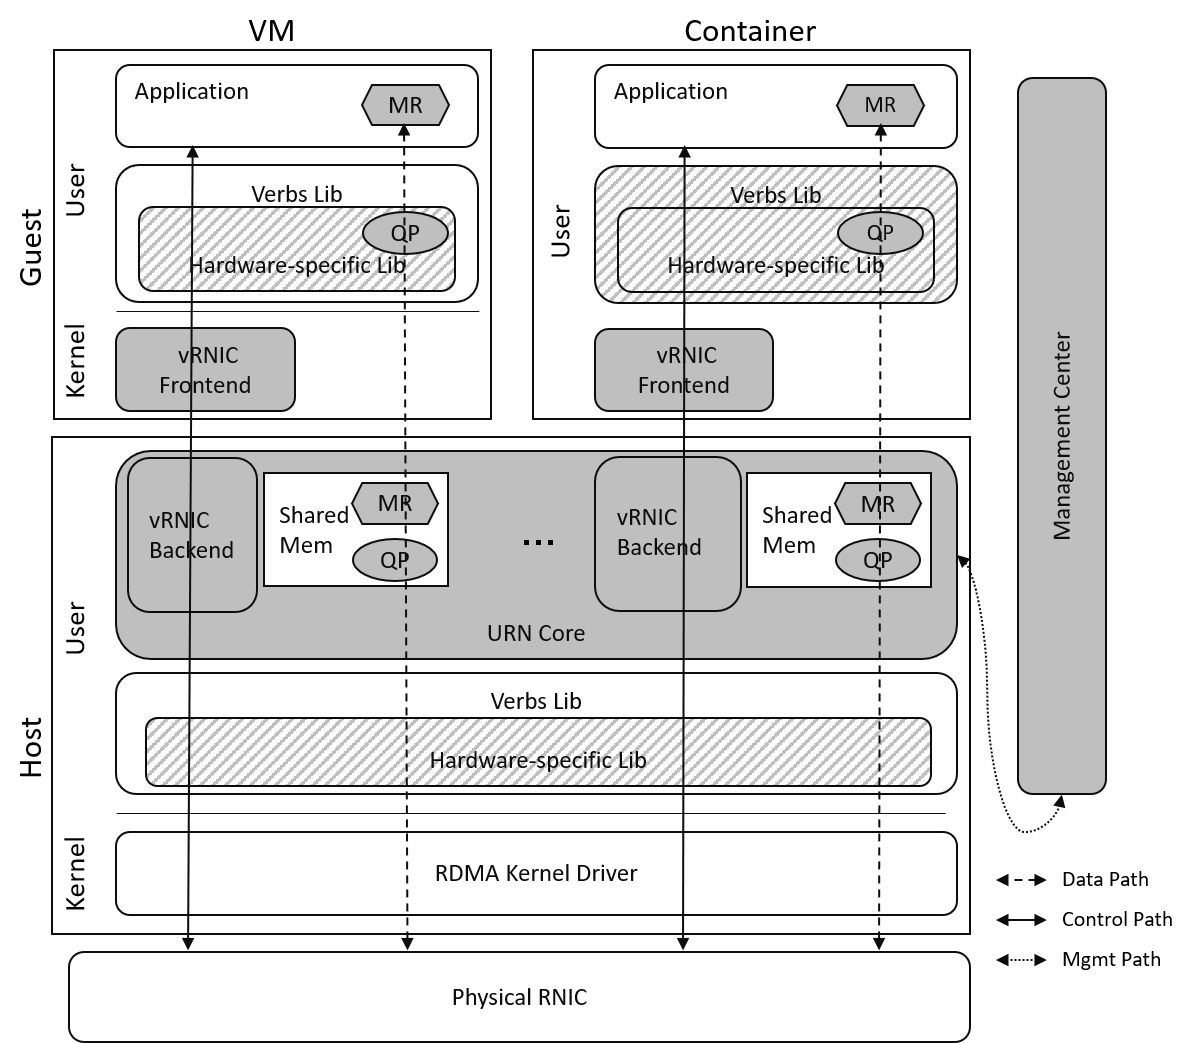
\includegraphics[width=1\linewidth]{images/framework-overview.png}
	\caption{uniRDMA Framework Overview}
	\label{fig:framework-overview}
\end{figure}
\section{Design} \label{design}

The design goals of \sys are:
1) to provide a unified RDMA virtualization framework for the hybrid virtualization environment where VMs and containers co-exist on the same machine or in the same data center. Data center owners do not have to maintain two RDMA virtualization stacks. And a server can flexibly choose to host VMs or containers or both, without considering which RDMA virtualization stack is installed.
2) to provide a single point of RDMA resource management for all RDMA resource users so that the resources can be optimally scheduled.
3) to keep the performance overhead of the RDMA virtualization to the minimum.
4) It should bring minimum impact to existing RDMA software stack and be completely transparent to RDMA applications.

\begin{figure}[!ht]
	\centering
	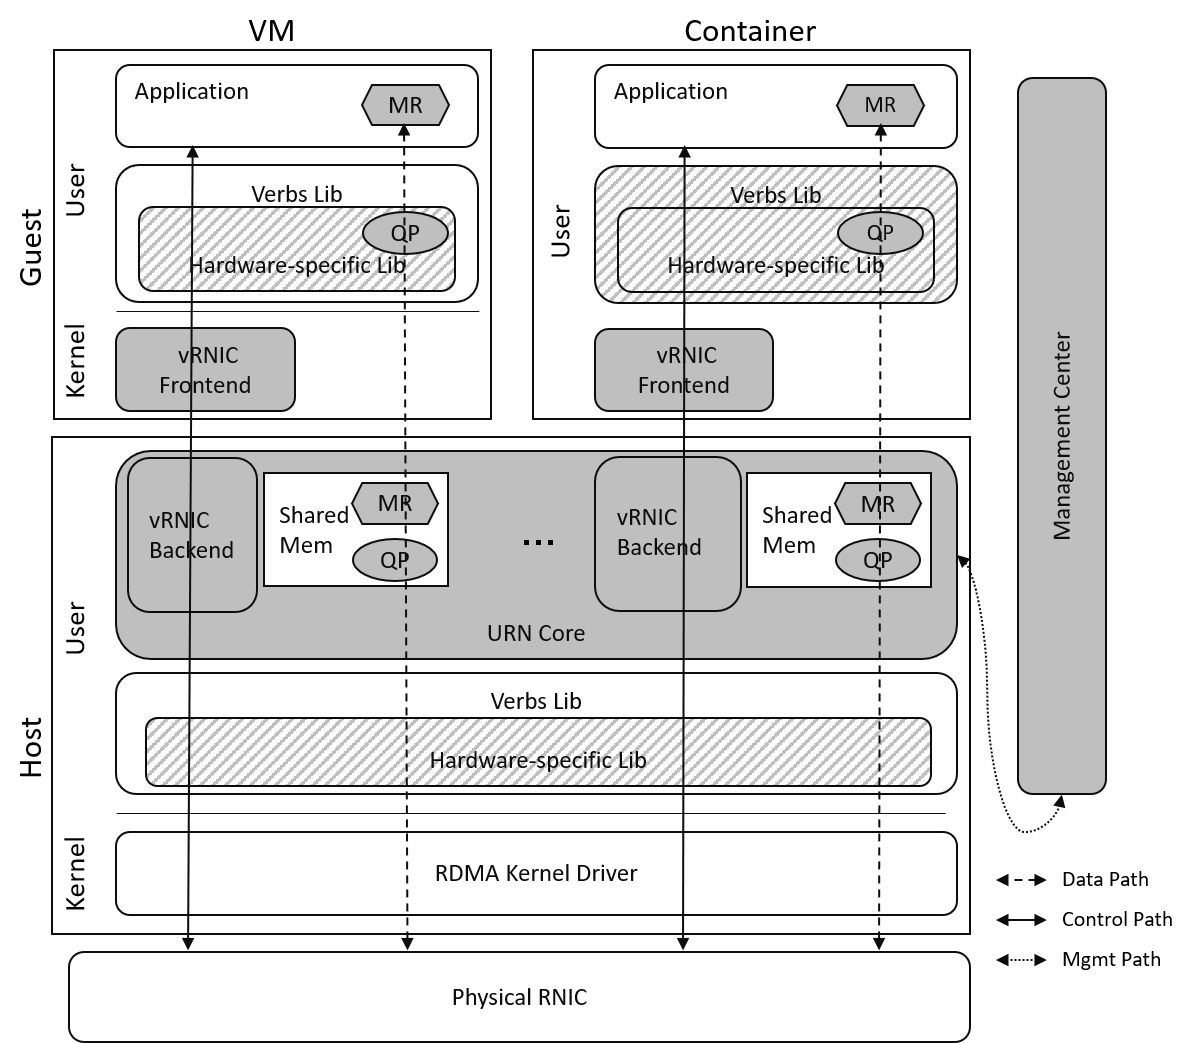
\includegraphics[width=0.8\linewidth]{images/framework-overview.png}
	\caption{Architecture overview of \sys. The light grey boxes are modules in \sys framework. The dark grey boxes are the memory shared by both the application and the \sys Core. The shared memory can also be directly accessed by the RNIC.}
	\label{fig:framework-overview}
\end{figure}

The architecture of \sys is shown in Figure~\ref{fig:framework-overview}.
\sys consists of three parts, the vRNICs, the \sys Core and the management node. vRNIC is a virtual RDMA network device that looks like a real RDMA device inside VMs and containers. \sys Core is a virtualization layer for centralized RDMA resource management on the host machine. And the management node is a centralized management entity in the data center that keeps and coordinates management and control policies for the RDMA network.
In addition, some modifications are made to the Verbs library and device userlib in the user-space of the host and the guest to adapt to \sys.

\subsection{vRNIC}

The vRNIC is a virtual RDMA device that consists of a frontend and a backend. The vRNIC backend is placed in the host space and emulates the behavior of an RDMA device. The vRNIC frontend is placed in the guest space that exposes RDMA device interfaces to the upper device drivers.
On the control path, commands are forwarded from the vRNIC frontend to the vRNIC backend to be actually executed or emulated.
On the data path, the key RDMA resources (e.g., QPs and MRs) are directly mapped by the RDMA applications in the guest environment to the physical RDMA device. During actual data transmission both vRNIC frontend and backend are bypassed.

%--------------------------------------------------------------------------------------------------------------------------
\subsubsection{\textbf{vRNIC Backend}}
\
\noindent

%\newline
The vRNIC backend is implemented as a user-space module in the host system, similar to vhost-user-net~\cite{vhost-user-net}. Compared to kernel-space, there are three advantages for a user-space backend: first, user mode backend can utilize the Verbs API, which is a stable abstraction layer; second, user mode programming is easier than that of kernel mode; third, the attack surface is limited to user-space with lower risk.

% vRNIC作为一个虚拟RDMA设备,vRNIC后端需要维护关于RDMA网卡的硬件属性,与物理RDMA网卡对应,例如RDMA地址vGID,RDMA设备类型等。此外,在vRNIC的运行过程中,vRNIC后端中需要维护三方面的上下文:
% 1,来自guest的虚拟RDMA上下文信息,主要记录了虚拟RDMA资源的信息;
% 2,由物理网卡创建的RDMA上下文,包含各RDMA资源,由vRNIC后端通过调用verbs库创建和维护;
% 3,虚拟RDMA上下文到物理RDMA上下文之间的对应关系。对应关系是一对一的,因为一对一是RDMA性能隔离的基础。

As a virtual RNIC device emulator, the vRNIC backend needs to maintain the same set of hardware properties that the physical RNIC has, such as the RDMA address GID. In addition, three kinds of contexts need to be maintained in the vRNIC backend at runtime:
1) Information of the runtime RDMA resources created and used on the emulated RDMA device, such as the memory address of the virtual MR/QP;
2) Information of the runtime RDMA resources actually created and used on the physical RNIC, such as the memory address of the real MR/QP;
3) The mapping between virtual RDMA context and physical RDMA context.

vRNIC backends are instantiated by the \sys Core.
The vRNIC backend acts like an RDMA application in the host environment and interact with physical RNIC through the Verbs library.

% 如果guest中所有RDMA操作均转发到vRNIC后端执行,将会引入额外上下文切换及数据拷贝,例如,MR中的数据内容或QP中的工作请求等,从而导致RDMA性能下降。考虑到控制路径仅涉及到初始化和连接建立的过程,其开销是一次性的,而数据路径是影响RDMA性能的关键。因此,为了提高RDMA网络性能,guest中RDMA资源与vRNIC后端完成了映射,数据路径直接使用映射的RDMA资源,其命令未转发到vRNIC后端。具体来说,vRNIC后端与guest共享了一些内存区域,vRNIC后端使用该共享内存创建RDMA资源并映射给上层的guest应用,包括MR、QP、CQ和DoorBell等。然后,guest应用基于这些映射的RDMA资源执行数据路径的操作,这些操作会被RDMA物理网卡执行,不用经过vRNIC后端和虚拟机内核。因此,避免了额外的数据拷贝和进程切换,从而实现了与原生RDMA相当的性能。

%精简一下,看下有没有和后面的workflow部分重复
When RDMA requests are forwarded from a vRNIC frontend to its backend, it causes context switching and data copy between the guest and the host. For example, when sending a data package, the data content in MR and the work request in QP need to be forwarded to the backend. This incurs performance degradation, especially on the data path. In order to achieve maximum performance, the RDMA resources are mapped in the shared memory region of the vRNIC backend and the RDMA application in the guest. On the data path, both the transmitted data and the sending/receiving requests are directly accessible to both the vRNIC backend and the RDMA applications, without an extra copy operation. Specifically, the vRNIC backend allocates RDMA resources in the shared memory region and the RDMA application in the guest environment maps to the same memory region in its own address space. The RDMA resources include MR, QP, CQ, and Doorbell. The RDMA application puts data and requests in the shared RDMA memory region. The physical RNIC sees the data transmission requests in the shared memory region and performs the actual work without involving the vRNIC backend and the guest OS kernel.

The design of the vRNIC backend is the same for VMs and containers.

%-----------------------------------------------------------------------------------------------------------------------------
\subsubsection{\textbf{vRNIC Frontend}}

\
\noindent

The vRNIC frontend is located in the guest environment acting as the NIC interface. Applications in the guest environment can use the NIC interface through Verbs library. For VMs, the frontend virtual device is in guest kernel space and is designed to expose interfaces the same way as the RDMA NIC device to the upper kernel device drivers. For containers, the frontend module is implemented as a library that is linked to the applications alongside with Verbs library.

% 在虚拟机或容器中,vRNIC前端都是连接虚拟机或容器应用到vRNIC后端,但是它们的设计上有差别。 
% 在虚拟机场景中,vRNIC后端模拟了一个外部设备,由虚拟机OS中的vRNIC前端驱动。原生RDMA内核驱动包括与设备无关的OFED模块和设备相关的模块,OFED模块接收verbs操作并转化为内核层级的RDMA 命令;设备相关模块注册具体接口到OFED,并通过物理RNIC执行这些调用。对应的,在虚拟机中为了使用vRNIC,一个自定义的设备相关的驱动模块被构建在虚拟机内核,用来提供与原生类似的设备相关接口并注册它们到OFED模块。OFED中的RDMA命令将通过这些设备相关接口,被转发到vRNIC前端模块,再从前端转发到vRNIC后端去执行。因此,原生的RDMA应用无需修改便可运行在虚拟机中,而且虚拟机内核仍然可以使用RDMA (and RDMA can be used in the guest kernel)。
% 在容器场景中,应用和vRNIC后端共享主机内核,仅位于不同的命名空间。为了在容器中使用vRNIC,容器的verbs库中与内核RDMA驱动交互的接口,被替换为vRNIC前端接口。Verbs操作被劫持到vRNIC前端,并被转发到vRNIC后端。

For both VMs and containers, the vRNIC frontend in the guest connects to the vRNIC backend in the host, but in different ways.
For VMs, the native RDMA software stack is kept including the Verbs and device-specific library in the user space, and the OFED and hardware-specific driver in the kernel space. However, the hardware-specific device driver is connected to the vRNIC frontend instead of a physical RNIC. As shown in Figure~\ref{fig:framework-overview}, the hardware-specific device driver is replaced by a \sys version of thin device driver that is registered to OFED core. In this way, RDMA requests in the VM are re-routed to the vRNIC.
For containers, as shown in Figure~\ref{fig:framework-overview} the Verbs library is hijacked to interact with the vRNIC instead of the orignal kernel RDMA driver by replacing the file descriptor of physical RNIC with one of vRNICs~\cite{kim2019freeflow}.

In both VMs and containers, the changes in RDMA software stack are totally transparent to RDMA applications.


%--------------------------------------------------------------------------------------------------------------------------
%--------------------------------------------------------------------------------------------------------------------------
%--------------------------------------------------------------------------------------------------------------------------
\subsection{\sys Core}

Each machine is designed to have one \sys Core instance in its host user space. The \sys Core is designed to manage both the virtual and physical RDMA resources for the host. It instantiates vRNIC backends, manages virtual RDMA network configurations and policies, and interact with physical RNIC through the Verbs library.

% 为了对vRNIC进行统一管理,高效利用物理RDMA网卡,我们构建了一个统一的虚拟层\sys Core。\sys Core部署于集群的每台服务器上,监听虚拟机、容器以及原生的RDMA设备请求。之后,在\sys Core中实例化vRNIC和配置虚拟RDMA网络等。

%【 讨论:管理服务器的所有RDMA资源,对于来自虚拟机和容器的网卡资源申请,\sys Core会进行。1,发现和记录所有RDMA资源, 2,监控RDMA资源消耗,决策RDMA设备和资源分配(调度方式:动态轮询等等,调度目的:负载均衡、控制资源QoS),3,RDMA虚拟机容器的迁移信息】

%--------------------------------------------------------------------------------------------------------------------------
%\subsubsection{\textbf{\sys Core Service}}
%\
%\noindent

% \sys Core 作为一个服务会在每台服务器上运行,统一监听虚拟机、容器和主机的获取RDMA设备的请求(如果原生的请求不进行统一处理,将会导致原生和虚拟化对RDMA设备接口的冲突,因此修改了主机获取设备Verbs ibv_get_device_list的实现,将对应请求转发到\sys Core,由\sys Core统一分配RDMA设备接口)。

The \sys Core is deployed on each server listening to the request of RDMA device from VMs, containers and the RDMA applications in the host environment. To overtake the management work of all RDMA resources, the implementation of the Verbs \texttt{ibv\_get\_device\_list} is modified so that the corresponding request is forwarded to the \sys Core. The vRNICs are instantiated and configured by the \sys Core.

%The \sys Core as a service which runs on each server and monitors the request of obtain RDMA devices from VMs, containers and host. (If the host requests are not processed uniformly, it will cause the RDMA devices interfaces conflict between host RDMA and virtualized. So the implementation of the verbs ibv\_get\_device\_list is modified, the corresponding request is forwarded to the \sys Core, and the \sys Core uniformly allocates the RDMA device interface) .

%--------------------------------------------------------------------------------------------------------------------------
\subsubsection{\textbf{Instantiating vRNICs}}
\
\noindent

% \sys Core在收到guest中应用申请vRNIC的请求后,会实例化vRNIC。实例化vRNIC的主要工作包括: 初始化vRNIC属性、绑定vRNIC到物理网卡、构建vRNIC前后端消息通道以及隔离各vRNIC实例等。

Instantiating vRNIC mainly includes 3 steps: 1) initializing vRNIC attributes; 2) binding the vRNIC to the physical RNIC; 3) building the message channel between the vRNIC frontend and backend.

% 初始化vRNIC属性:为了模拟与硬件一致的功能接口,\sys Core需要对vRNIC的不变属性进行初始化,包括RDMA地址vGID,设备号等等。对于RDMA地址vGID,\sys Core会随机生成IPv6格式的虚拟值,同时登记到mgmt center的数据库中。

1) Initializing vRNIC attributes: To emulate a physical RNIC, \sys Core needs to initialize the static properties of vRNIC, such as RDMA address vGID and device number. For RDMA address~(vGID), \sys Core randomly generates the values in the IPv6 format and registers them into the database in the management node.

% 绑定vRNIC到物理网卡:vRNIC实例需要依靠物理网卡实现RDMA功能,因此,实例化vRNIC时需要将vRNIC实例与对应的物理RDMA网卡绑定。如果是多网卡设备或者多个网卡接口(如使用SR-IOV),还需确定从vRNIC到对应物理网卡接口的映射关系。

2) Binding vRNIC to the physical RNIC: \sys Core binds the vRNIC instance to the physical RNIC when instantiating. If there are multiple physical RNICs or RNIC interfaces~(e.g., Virtual Functions), the \sys Core needs to have a resource allocation algorithm, taking into consideration of the network topology and network load balance.

% 构建vRNIC消息通道:\sys Core需要构建vRNIC后端与vRNIC前端之间的消息通道。对于容器来说,容器与vRNIC后端共享某一IPC命名空间,即可完成vRNIC前端与后端之间的消息交互。对于虚拟机来说,由于vRNIC后端在主机用户空间,而hypervisor位于主机内核空间。为了避免guest的消息先拷贝到hypervisor层再到vRNIC后端,我们构建一块共享内存,以此作为消息通道。具体来说,虚拟机物理内存与vRNIC后端之间是共享的。guest中的任意RDMA消息,均可以直接由vRNIC后端获取,同时也减少了从guest到vRNIC后端的延迟。

3) Building the vRNIC message channel: \sys Core needs to build a message channel between the vRNIC backend and the frontend.
For containers, the container can share an IPC namespace with the vRNIC backend as the message channel.
For VMs, to avoid the two-hops memory copy from the vRNIC frontend in the guest to the hypervisor and then to the vRNIC backend, we use the shared memory as the message channel. Specifically, the physical memory in the VM is shared with the vRNIC backend. RDMA messages in the guest can be directly accessed from the vRNIC backend.

%--------------------------------------------------------------------------------------------------------------------------
\subsubsection{\textbf{Configuring the Virtual RDMA Network}}
\
\noindent

% \sys Core在实例化vRNIC后,需要对vRNIC的网络进行配置,包括虚拟RDMA地址配置以及虚拟RDMA路由配置。
After the instantiation of the vRNIC, the \sys Core needs to configure the vRNIC's network, including virtual RDMA address and virtual RDMA routing.
For virtual RDMA address configurations, the vGID assigned to the vRNIC by \sys Core is a logical value, independent of the physical RNIC, when it instantiates the vRNIC.
% 对于虚拟RDMA地址配置,\sys Core 在实例化vRNIC时, 给vRNIC配置的vGID是虚拟值,与物理网卡无关。

% 对于虚拟RDMA路由配置,每台主机的\sys Core中配置了虚拟RDMA网络路由规则。具体来说,\sys Core在实例化vRNIC时,还给每个vRNIC都配置了组ID,路由规则的定义形式为:{group ID1, group ID2, Policy}。例如,如图4所示,容器1和容器2的vrnic被配置到同一组中,因此允许创建RDMA连接。作为对比,容器1和虚拟机1属于不同的用户组,按路由规则无法建立RDMA连接。各虚拟实例之间建立RDMA连接的具体细节可以参考4.3.1。

For virtual RDMA routing configurations, virtual RDMA network routing rules are configured in the \sys Core at each host. In specific, \sys Core also configures the group ID for each vRNIC when it instantiates the vRNIC. Routing rules are defined as \{group ID1, group ID2, Policy\}. For example, as shown in Figure \ref{fig:route-config}, the vRNIC of container 1 and container 2 are configured into the same group, thus allowing RDMA connections to be created. In contrast, container 1 and VM 1 belong to different user groups and cannot establish an RDMA connection according to routing rules.

% RDMA与传统TCP/IP不同,RDMA还支持单边操作。在guest应用的RDMA单边操作中,RDMA的工作请求中包含了远端的GVA及key,远端MR内存地址同样需要在RDMA用户态驱动中转换为远端vRNIC后端的HVA。为了便于远端地址的转换,我们在\sys Core中建立了一个分布式的Key-Value数据库,存储各节点注册MR的映射关系{key,gva, hva}。在guest应用执行单边操作时,将向\sys Core 中的分布式KV数据库查询,以获取远端MR的HVA,缓存到本地并在写入工作请求以前。

Unlike traditional TCP/IP network, RDMA networks also support one-sided operations. The remote Guest Virtual Address~(GVA) and key is included in the one-sided work request, and the GVA also needs to be translate to the remote Host Virtual Address~(HVA) by the RDMA application. To facilitate the remote memory address translation, we set up a distributed key-value database in the \sys Core to store the mapping between GVA and HVA for each registered MR using tuple~\textit{\{Host, MR-KEY, GVA, HVA\}}. When the application in the guest performs a one-sided operation, it will query the distributed key-value database in the \sys Core for the remote HVA of the MR, and caches it locally.

% 总之,\sys Core中的虚拟网络配置是动态调整的,因此,容器和虚拟机迁移后无需更改物理网卡及交换机等硬件的网络配置,实现便携的虚拟机或容器迁移。基于\sys Core中的虚拟路由规则,可以支持云环境中的多租户隔离。而各\sys Core存储的MR地址映射关系,对单边操作给予了支持。

%In summary, the virtual network configuration in the \sys Core is dynamic, so it is unnecessary to change the network configuration of hardware such as the physical RNICs and switches to enable portable VM or container migration. Based on virtual routing rules in the \sys Core, multi-tenant isolation in a cloud environment can be supported. The MR memory mapping is recorded at each \sys Core to support one-sided operations.

\begin{figure}[!ht]
	\centering
	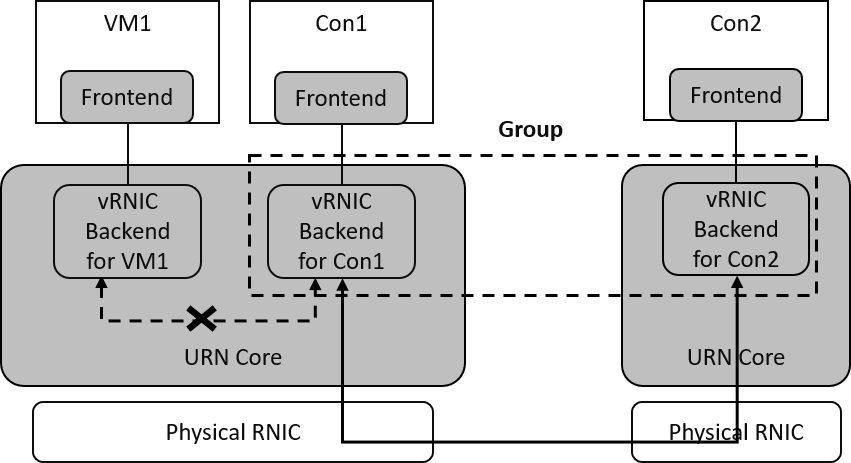
\includegraphics[width=0.75\linewidth]{images/route-config}
	\caption{RDMA group configuration and routing. The vRNICs of container 1 and container 2 are configured in the same group. Thus, the two containers are allowed to create RDMA connections. VM 1 is not in the same group of the containers. So it is not allowed to create RDMA connections to the containers.}
	\label{fig:route-config}
\end{figure}


%------------------------------------------------------------------------------------------------------------------------------------------
%-----------------------------------------------------------------------------------------------------------------------------------------
%-----------------------------------------------------------------------------------------------------------------------------------------
\subsection{Management Node}

In \sys, there is one centralized management node in the cluster that manages the control policies of the entire RDMA network, e.g., ACL and QoS.

% 在\sys框架里,整个集群配备一个mgmt center,作为配置管理,存储各节点RDMA资源信息的中心。
%In \sys, the cluster is equipped with one management node, which serves as configuration management and stores the information of RDMA resources for each node.

% 通过mgmt center,管理者向各个节点的\sys Core下发各种策略,包括控制平面策略,如连接管理,防火墙等;和数据平面策略,如Qos、流量计费等。管理框架图如图5所示:策略由mgmt center下发到\sys Core,\sys Core通过agent接收策略后,其中,\sys Core将控制平面策略配置给管理的各vRNIC后端。对于数据平面策略,\sys Core将其发送给 Verbs库中的agent,然后在各虚拟机的RDMA应用本地执行。

Through the management node, policies are issued to the \sys Core on each node, including: control plane policies, such as connection management, firewall, etc;  and data plane policies, such as QoS, traffic metering, etc. The management framework is shown in Figure~\ref{fig:mgmt-center}. The \sys Core receives the policies through an agent. Then, the \sys Core configures the control plane policies for each managed vRNIC backend.
For the data plane, the \sys Core synchronizes the policies with the agent in the Verbs library in the guest environment.
Note that this design requires \sys to trust the Verbs library in the guest environment. That means the Verbs library in the guest environment is included in the TCB~(Trusted Computing Base). Compared with native RDMA stack, its data path bypasses the OS kernel. The policies are also enforced by the Verbs library.

%  连接管理、防火墙等控制平面策略主要基于RDMA连接进行,依靠QP等RDMA资源。由于包括QP在内的所有RDMA资源均已经映射在vRNIC后端中,因此,控制平面策略可以直接在vRNIC后端依靠映射的RDMA资源执行;数据平面策略也可以依靠轮询各vRNIC后端的映射好的RDMA资源来完成。然而,这样做将消耗额外的CPU资源而且可能不正确如果轮询效率不高。因此,本文将数据策略进一步从\sys Core下发到各guest的用户库,在各RDMA应用本地执行。注意,这些扩展需要所有客户机都信任库,并且这些修改应该包含在TCB(可信计算库)中。对照native的RDMA,其数据路径绕过了操作系统内核,物理网卡的数据管理及其有限,因此,其细粒度的数据管理同样需要在应用本地执行,并需要Verbs库的帮助。

%The control plane policies are mainly about on RDMA connections, which rely on RDMA resources such as QP. Since all RDMA resources, including QP, are mapped to the vRNIC backend, the control plane policies can be executed in the vRNIC backend against the mapped RDMA resources. The data plane policies such as QoS also can be completed by polling the mapped RDMA resources in the vRNIC backend. However, the polling occupies additional CPU and may not be correct if polling is slow. Therefore, the data plane policies are further issued from \sys Core to each guest's user library, executed locally in each application. Note that these extensions require that the guest trusts its Verbs libraries, and that these changes should be included in the TCB(Trusted Computing Library). Compared with native RDMA, its data path bypasses the kernel, while the data management in physical RNIC is very limited. Therefore, the fine-grained data management of RDMA also needs to be executed locally in application with the help of the Verbs libraries.

\begin{figure}[!ht]
	\centering
	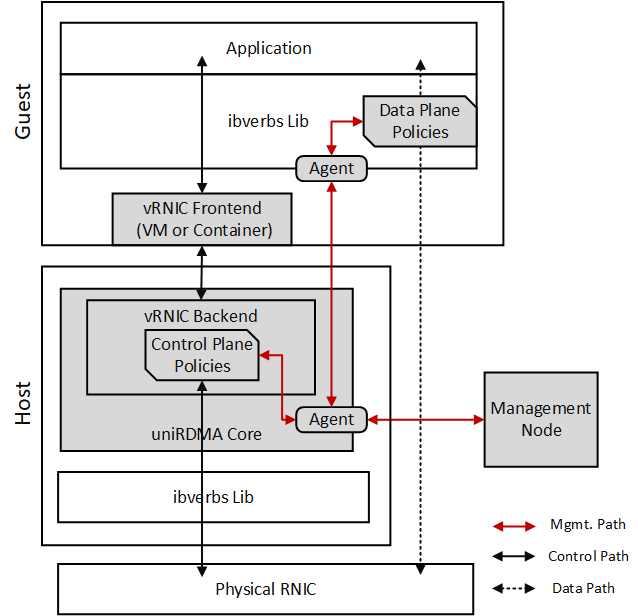
\includegraphics[width=0.75\linewidth]{images/mgmt-center.png}
	\caption{The architecture of \sys management plane}
	\label{fig:mgmt-center}
\end{figure}


%------------------------------------------------------------------------------------------------------------------------------------------
%-----------------------------------------------------------------------------------------------------------------------------------------
%-----------------------------------------------------------------------------------------------------------------------------------------
\subsection{Verbs and User-space Device Library}

%% 两小节: 控制路径和数据路径
%% 给图
% Verbs库为RDMA应用提供了统一的Verbs接口,在控制路径上,Verbs库接受RDMA应用的Verbs命令并与RDMA内核驱动进行交互,在数据路径上,Verbs库调用设备相关用户态驱动,绕过了操作系统内核。为了让虚拟机或容器中的应用使用vRNIC,同时确保\sys对应用的透明性,Verbs库及其相关驱动需要适配vRNIC架构并提供与原生一致的Verbs接口。如图所示,针对控制路径和数据路径,在verbs库和用户驱动中有一些关键的修改工作。

\begin{figure*}[!ht]
	\centering
	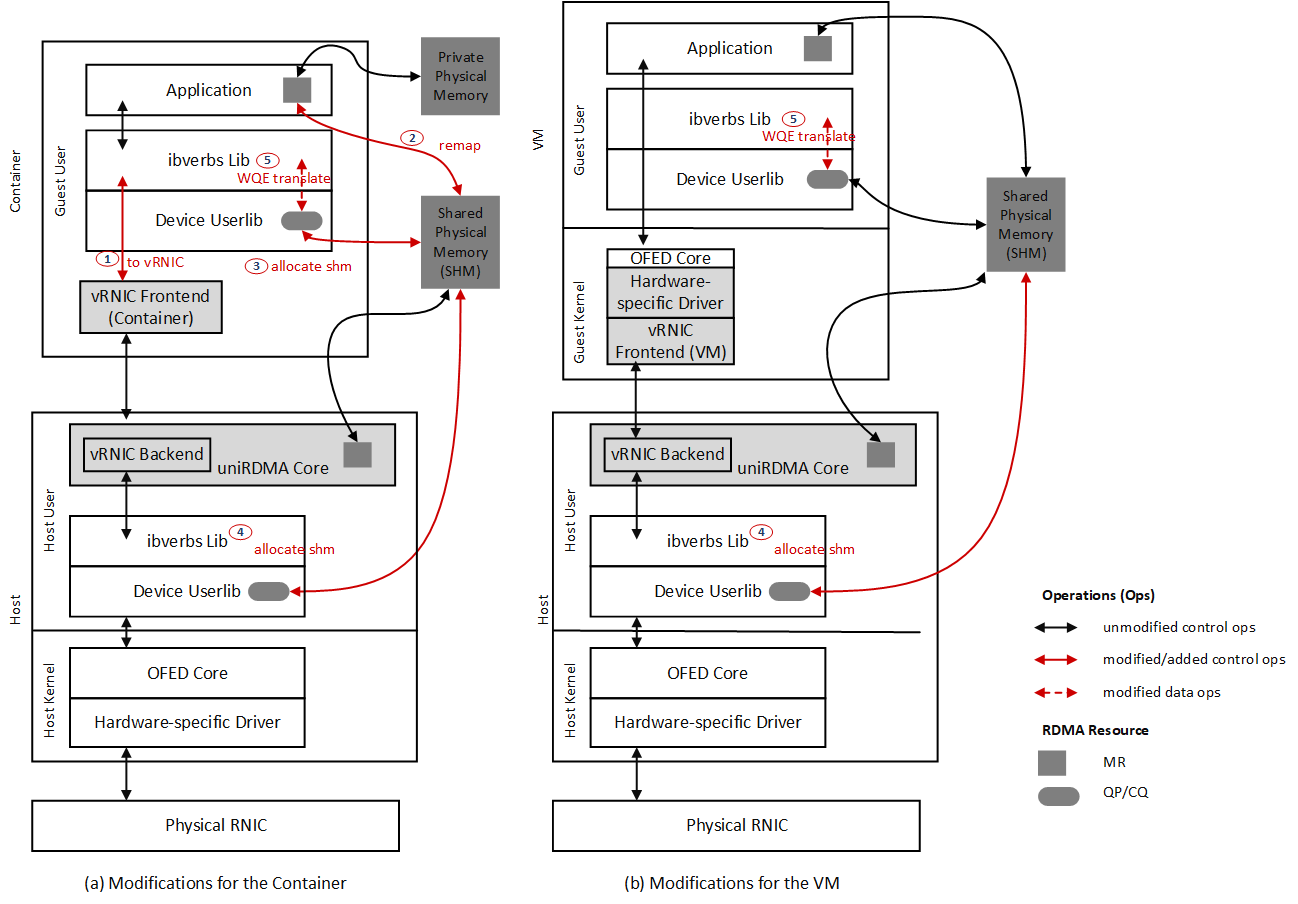
\includegraphics[width=0.72\linewidth]{images/verbs-driver}
	\caption{Modifications in the Verbs library and user-space device library for containers and VMs}
	\label{fig:verbs-driver}
\end{figure*}


The Verbs library provides the abstracted interface for the RDMA applications. In \sys, this interface is kept intact.
The Verbs library and the device library are modified so that they are redicted to use the vRNIC instead of the physical RNIC. As shown in Figure~\ref{fig:verbs-driver}, there are several modifications to the Verbs library and user-space device library on both control path and data path.


% 在容器中,为了让Verbs转发到vRNIC后端,将Verbs库中到内核驱动的接口替换为到vRNIC前端交互的接口,如图4-a-1所示。此外,为了让容器应用与vRNIC后端之间完成RDMA资源的共享内存映射,包括MR、QP/CQ和DoorBell,具体修改如下:
%(1)针对MR:在原生RDMA中,MR的buffer是由应用指定的,并且通常是私有内存。容器的Verbs用户库中将应用指定的MR内存重新映射到指定的共享内存,如图4-a-2所示。然后将该共享内存路径和GVA随Verbs命令及参数传递到vRNIC后端。vRNIC后端可以利用这一共享内存创建MR, 并将GVA传递到RDMA内核驱动,由RDMA内核驱动缓存给物理网卡。
%(2)针对QP/CQ:原生RDMA中QP/CQ内存的分配是在用户态驱动中进行的,也不是共享内存。在容器的用户态驱动中分配共享内存作为QP/CQ buffer,如图4-a-3所示。对应的共享内存信息会随Verbs命令和参数传递到vRNIC后端。
% vRNIC后端在创建QP/CQ时,将分配这一共享内存作为QP/CQ的buffer,如图4-a-4所示。

On the control path, the modifications are different for containers and VMs.
For the containers, to forward the Verbs calls to the vRNIC backend, the Verbs library is hijacked to use the file descriptor of the vRNIC backend instead of the original RNIC file descriptor, as shown in Figure~\ref{fig:verbs-driver} (a)-1. In order to achieve high performance, the memory of the RDMA resources are mapped by both the application and the vRNIC backend~(including MR, QP/CQ and Doorbell). Modifications are introduced in the Verbs library and user-space device library as follows:

1) MR: In native RDMA, the MR buffer is assigned by the application and is private.
In \sys, the container's Verbs library will remap the GVA~(Guest Virtual Address) of the MR buffer to the shared physical memory, as shown in Figure~\ref{fig:verbs-driver} (a)-2. And the GVA of the shared memory will be forwarded to the vRNIC backend. The vRNIC backend register the MR using the GVA by calling the RDMA kernel driver~(OFED).

2) QP/CQ: In native RDMA, the QP/CQ buffer is allocated by user-space Verbs library and is private.
In \sys, the container's user-space Verbs library allocates QP/CQ buffer in the shared memory region, as shown in Figure~\ref{fig:verbs-driver} (a)-3. The GVA of the shared memory will be forwarded to the vRNIC backend. When the vRNIC backend creates QP/CQ, it will register the QP/CQ using the GVA of the shared memory, as shown in Figure~\ref{fig:verbs-driver} (a)-4.

%(3)针对DoorBell:在原生RDMA中,verbs库打开RDMA设备接口,经RDMA内核驱动映射门铃到应用程序。在\sys中,Verbs库打开虚拟的设备接口,并通过vRNIC后端和内核辅助模块来映射门铃。具体细节在第5节介绍。

3) DoorBell: In native RDMA, the RDMA device is opened in the Verbs library and DoorBell is mapped to the applications through the RDMA kernel driver.
In \sys, the container's Verbs library opens the virtual device interface and maps the DoorBell through the vRNIC backend. %The details will be introduced in Section \ref{impl}.

% 在虚拟机中,vRNIC在实例化时已经共享了虚拟机的整块物理内存空间。即使虚拟机应用使用默认的方式分配MR、QP或CQ等RDMA资源的内存,无需修改,vRNIC后端可以获取对应的共享内存块。具体地,通过虚拟机内核的vRNIC前端驱动中,将这些buffer的GPA(虚拟机物理内存信息)随RDMA命令和参数转发给vRNIC后端,vRNIC后端可以将GPA翻译为HVA,并使用这些共享内存块作为RDMA资源MR,QP或CQ的buffer,如图4-b-4所示。

%这是KVM实现的个例
For the VMs, \sys maps the whole physical memory of the VM to the memory space of the corresponding vRNIC backend.
The RDMA applications in the VM allocate the memory for MR, QP and CQ. Then, through the vRNIC frontend, the GPA~(Guest Physical Addresses) of these memory buffers can be forwarded to the vRNIC backend. The vRNIC backend can translate the GPA to the HVA~(Host Virtual Address) in its own address space and gain the access to the memory of MR, QP and CQ, as shown in Figure~\ref{fig:verbs-driver} (b)-4.

% 基于上述修改,在数据路径上,无论是虚拟机还是容器,数据Verbs操作不需要转发到vRNIC后端,可以直接在guest用户空间,和原生RDMA一样避免了径额外的的拷贝或切换开销。

Based on these modifications, for both VMs and containers on the data path, the direct data delivery channel is established between the RDMA application in the guest user-space and the physical RNIC. It avoids the overhead of data copy or context switches.


%------------------------------------------------------------------------------------------------------------------------------------------
%-----------------------------------------------------------------------------------------------------------------------------------------
%-----------------------------------------------------------------------------------------------------------------------------------------
\subsection{Virtual RDMA Workflow}

% 图4说明了虚拟RDMA的详细工作过程。虚拟RDMA的工作流程涉及guest中的应用、verbs库以及主机的vRNIC后端交互。整个工作流程依次分为初始化阶段、连接阶段和数据阶段。其中,初始化阶段分别包括设备打开和RDMA资源创建,连接阶段中RDMA应用通过QP与远端建立连接。数据阶段中RDMA应用执行数据路径的操作。

Figure~\ref{fig:rdma-path} illustrates the detailed workflow of \sys. The workflow involves the application, the Verbs library~(including the user-space device library and the vRNIC frontend) in the guest environment, and the vRNIC backend in the host environment.
The whole workflow can be divided into the initialization phase, the connection phase and the data phase. The initialization phase includes device opening and RDMA resource initialization.
In the connection phase, the RDMA application establishes a connection with the remote entity through QP.
In the data phase, the RDMA application performs the data sending and receiving operations.

\begin{figure}[!ht]
	\centering
	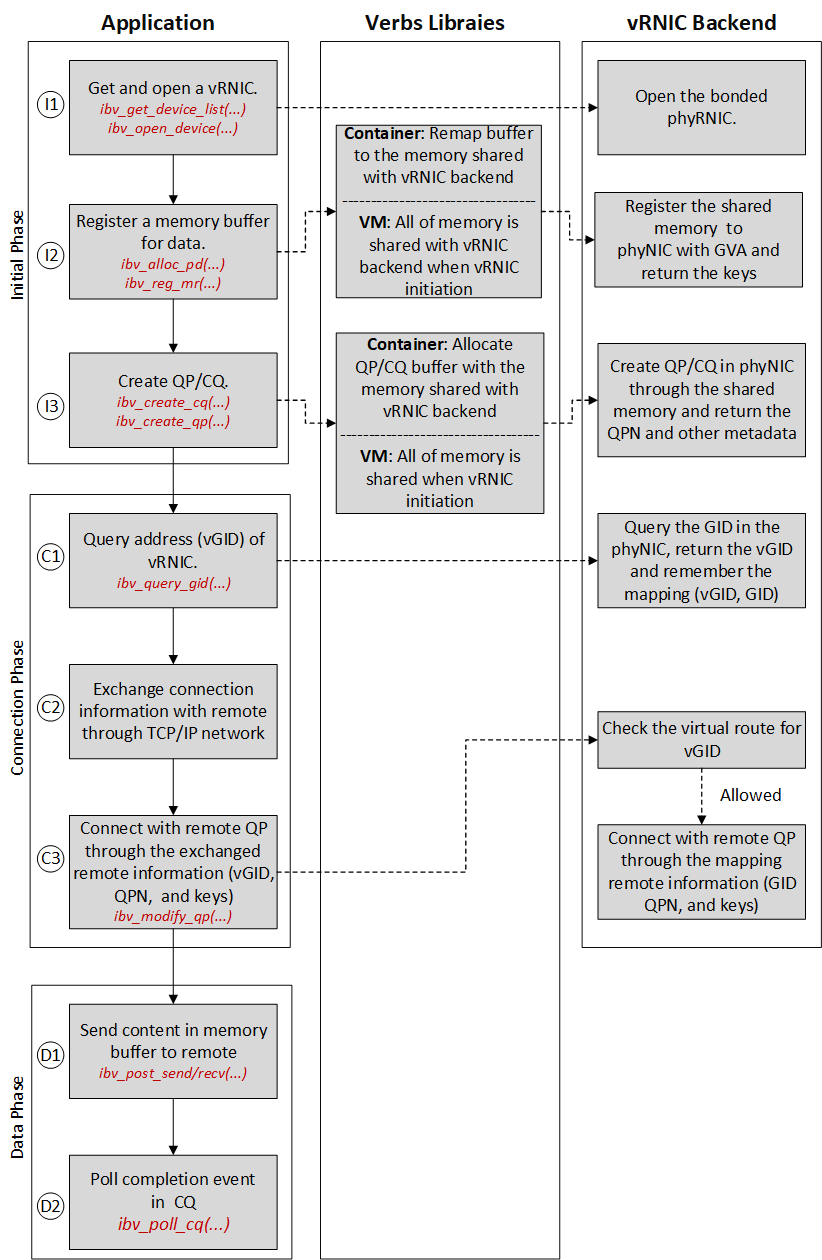
\includegraphics[width=0.95\linewidth]{images/RDMA-path.png}
	\caption{The Workflow of \sys SEND operation}
	\label{fig:rdma-path}
\end{figure}

% 4.4.1 初始化阶段
%  初始化阶段主要完成资源的初始化,分别包括设备打开(I1)、注册内存buffer(I2)和创建QP/CQ等RDMA资源(I3)。具体细节如下: 

%------------------------------------------------------------------------------------------------------------------------------------------
\subsubsection{\textbf{Initialization Phase}}
\
\noindent

Initialization stage is mainly about the initialization of resources, including vRNIC device opening~(I1), MR registration~(I2) and QP/CQ creation~(I3). The details are as follows:

% I1(Guest应用打开vRNIC设备):Guest应用依次调用Verbs接口ibv_get_devicelist和ibv_open_device,获取并打开vRNIC设备。这些调用会被劫持到vRNIC后端,vRNIC后端将打开在vRNIC实例化时绑定的物理RDMA设备。

I1 (vRNIC Device Opening): The application gets and opens the vRNIC device by calling the Verbs \texttt{ibv\_get\_device\_list} and \texttt{ibv\_open\_device} APIs. The calls will be delivered to the vRNIC backend, which will open the corresponding physical RNIC.

% I2(Guest应用注册MR):在容器中,Verbs库中将MR buffer重新映射到某一共享内存,虚拟机无需此步骤, 因为当虚拟机启动时,整个虚拟机的内存已经被设置为共享的。vRNIC后端会获取对应的共享内存,并使用它来注册MR,并返回MR keys等信息。

I2 (MR Registration): For the containers, the Verbs library remaps the MR buffer to a shared memory region. This step is not required for the VMs, because the whole physical memory of the VM is shared with the vRNIC backend in \sys. The vRNIC backend registers the MR to the RNIC and gets the MR keys returned by the \texttt{ibv\_reg\_mr}.

% I3(Guest应用创建QP/CQ):在容器中,Verbs库使用共享内存分配QP/CQ buffer,虚拟机无需此步骤。vRNIC后端将获取对应的共享内存,并分配它为QP/CQ的buffer,并会返回QPN, CQN等元数据。 

I3 (QP/CQ Creation): For the containers, the Verbs library allocates QP/CQ buffers in the shared memory region. Similar to I2, for the VMs, the Verbs library allocates QP/CQ buffers in its original way. In \sys, the whole physical memory of the VM is shared with the vRNIC backend, including the QP/CQ buffers. The vRNIC backend creates QP/CQ for the physical RNIC using the same QP/CQ memory allocated by the Verbs library in the guest.

%4.4.2 连接阶段

%------------------------------------------------------------------------------------------------------------------------------------------
\subsubsection{\textbf{Connection Phase}}
\
\noindent
% 连接阶段表示RDMA基于QP建立连接,依次包括查询GID(C1)、交换连接信息(C2)和基于QP建立连接(C3),具体细节如下:

In the connection phase, the RDMA connection is established based on QP. It includes querying GID~(C1), exchanging connection information~(C2) and establishing connection~(C3). The details are as follows:

% C1(获取GID):Guest应用调用Verbs ibv_query_gid,请求获取vRNIC的vGID地址。vRNIC后端将获取绑定的物理RDMA网卡的GID,记录(vGID,GID)对应关系, 并返回vGID给应用。 
C1 (Querying GID): The application calls Verbs API \texttt{ibv\_query\_gid} to get the vGID of the vRNIC. The vRNIC backend will query the GID of the corresponding physical RNIC, record the mapping tuple \textit{\{vGID, GID\}} and return the vGID to the frontend.

% C2(交换连接信息):应用与远端交换建立连接所需的信息vGID,QPN和MR key等。 该步骤完全由应用独立完成。例如,应用中可以使用TCP/IP 或RDMA-CM来交换信息。
C2 (Exchanging Connection Information): The applications exchange the connection information, such as vGID, QPN and MR-key, with the remote entity. This step is done by the applications without the participation of \sys. For example, the application can use TCP/IP or RDMA-CM to exchange the information.

% C3(连接建立):应用调用verbs ibv_modify_qp 并将本地/远端的vGID、QPN等作为参数。该命令转发到vRNIC后端后,vRNIC后端会先根据\sys Core的路由表规则进行判断,如果允许,就会将本地/远端 vGID转换为对应的GID,再根据QPN,在两个vRNIC后端的QP间建立RDMA连接。
C3 (Connection Establish): The application calls the Verb API \texttt{ibv\_modify\_qp} with the parameters, including local/remote vGID and local/remote QPN. The vRNIC backend will check the routing table from \sys Core. If allowed, the local/remote vGID will be converted to GID, and RDMA connection is established based on local/remote QP in two vRNIC backends through the QPN.

% 4.4.3 数据阶段
% 数据路径发生在连接建立后,主要是对本地/远端 MR中的内容执行收发操作,包括图中的D1(收发数据)和D2 (轮询CQ)。具体如下:

%------------------------------------------------------------------------------------------------------------------------------------------
\subsubsection{\textbf{Data Phase}}
\
\noindent

The data phase is about how to send/receive the data in the local/remote MR buffers. It includes D1~(Send/Recv Data) and D2~(Poll the CQ). The details are as follows:

% D1(收发数据):在双边操作中,两端应用分别执行Verbs ibv_post_recv和ibv_post_send对本地MR中的数据进行收发。在单边操作中,仅执行ibv_post_send。

D1 (Send/Recv Data): For two-sided operations, the data in the local MR can be sent and received by executing Verbs APIs \texttt{ibv\_post\_recv} and \texttt{ibv\_post\_send}, respectively. For one-sided operations, only \texttt{ibv\_post\_send} is used.

% D2(轮询CQ):Guest应用轮询CQ来获取对应的工作完成通知。如果使用事件通知机制,guest中verbs库将等待vRNIC后端获取事件并返回给应用。

D2 (Polling the CQ): The application polls the CQ for the work completion. If event-based notification is used, the Verbs library will wait for the vRNIC backend to receive the event and return it to the application.

%\section{Implementation}
%我们在Linux环境中实现了\sys框架:
 We implement a prototype for \sys in Linux environments. The hypervisor of VM is QEMU/KVM and the container engine is Docker. The vRNIC frontend for VMs and containers is implemented differently. The \sys core (with vRNIC backends) includes about 2000 lines codes in the host user-space. And the management center is implemented through Zookeeper to the information for RDMA resources (such as RDMA address mapping, the numbers of VFs) and the policies (such as QP limit, QoS). In addition, we modified the Verbs library libibverbs-41mlnx1, the library about connection management librdma-cm, and the user-space RNIC driver libibverbs-41mlnx1. And we do some necessary work in host kernel, such as caching GPA into RNIC, mapping DoorBells. In this section, we introduce some representative implementation details:
 
 % 资源映射:根据资源所属于的物理地址空间,RDMA通信过程中主要有两类资源:内存资源(QP等),和设备资源(门铃).
 \subsection{Resource Mapping}
According the physical address space, there are mainly two kinds of resources for RDMA: memory resources (e.g. QPs, MRs) and device resources (e.g. DoorBells). 
 
 % 对于内存资源: 在虚拟机中, 我们利用vhost-user的半虚拟化技术构建vRNIC后端,vRNIC后端可以与虚拟机共享整块内存。 在具体操作中,需要先借助vRNIC前端将GVA转换为GPA;然后,在vRNIC后端中,由于vRNIC后端已经和虚拟机共享整块内存,因此,GPA可以被线性转换为HVA。但是,从GVA到GPA的转换由于guest OS的内存管理, 可能存在非线性的不连续现象,进一步导致vRNIC后端中映射的HVA区域也是不连续的。此时,在后端可以利用mremap系统调用重新映射虚拟内存,以将对应的物理页面映射到连续的HVA区间.
 For memory resources (e.g. QP), the mapping in VMs is as shown in Figure \ref{fig:qp-map}. We set the whole memory of the guest is shared in QEMU process, and the shared memory file path is registered in the vRNIC backend process. Because different processes can share the physical memory through the shared memory file. (1) The application in the guest allocate the QP buffer, and the buffer is using the shared memory in the host. The physical pages in the guest is pinned in the guest kernel. (2) The vRNIC backend receive the GPAs of the QP buffer. Note that the GPAs may not be contiguous. If we directly map the shared memory file through dis-contiguous GPAs (offsets), the obtained HVA also be dis-contiguous and cannot be used as the QP buffer. Thus, the vRNIC backend remap the corresponding shared memory to a new contiguous virtual memory region, and use it as the QP buffer.
 
 The mapping in containers is simple: The application in containers explicitly allocate the shared memory as the QP buffer in the modified Verbs libraries. Note that each QP, QP or MR uses a unique shared memory file. The vRNIC backend directly use the mapped region from the corresponding shared memory file.
\begin{figure}[!ht]
	\centering
	\includegraphics[width=1\linewidth]{images/qp-map.png}
	\caption{QP Mapping}
	\label{fig:qp-map}
\end{figure}

 

 For RDMA device resources (e.g. DoorBells), the mapping in VMs is as shown in  Figure \ref{fig:db-map}. (1) The application in the guest request the DB-HPA handle to the vRNIC backend. There are two reasons to do it: first, the page tables is different between the QEMU process (the guest) and the vRNIC backend processes, and the mapping from QEMU-HVA to DB-HPA must be done in QEMU process; second, the physical RDMA context is centrally maintained in the vRNIC backend, including the DB. (2) The application vRNIC backend receive the request and map the physical DoorBell. (3) The vRNIC backend obtain the DB-HPA handle through the helper module in the host kernel and return the handle to the application in the guest. (4) The vRNIC backend map a virtual DoorBell, forwards the GPA and DB-HPA handle to the helper module in the host kernel, and the helper module translate the GPA to QEMU-HVA. (5) The helper module remaps the QEMU-HVA to the DB-HPA. The helper module is implemented based on the para-virtrualization vhost modules, which provide high I/O performance  between the guest and the host kernel.
 
 In containers, the mapping of DoorBells is similar as the above. The only difference is that the application in the container directly forwards the virtual memory address to the helper module in the host kernel, through a simple costumed  character device driver. 
 \begin{figure}[!ht]
	\centering
	\includegraphics[width=1\linewidth]{images/db-map.png}
	\caption{DoorBells Mapping}
	\label{fig:db-map}
\end{figure}
 

\subsection{Register MR in the Host}
When vRNIC backend receives the registering MR commands and registers the MR, it should use the GVA as the virtual address when caching the page table for physical RNIC. And the physical RNIC can directly access the physical pages through the GVA in the work request of the application, instead of translating the GVA to the HVA in the data path. 

To implement it, we modified the OFED driver and the Verbs library in the host: the OFED driver can receive the GVA parameter when register MR, and fillwith the cached page table with the GVA as the virtual memory address.



\section{Evaluation} \label{eval}
In this section, we evaluate the performance of \sys based on the RDMA test tools and real applications. We expect to answer the following questions:

\begin{itemize}
\item How about the performance of \sys compared to that of native RDMA for both VMs and containers?
\item Can \sys be adapted to the real-world RDMA applications in both VMs or containers?
\end{itemize}

\subsection{Experiment Methodology}
All experiments are carried out on two servers. The settings mainly include three parts: host server, container and virtual machine. 

Each host server is equipped with 4 Intel Xeon E7-4850 2.40GHz 16-core CPUs and 1 TB RAM. The RNIC used is Mellanox ConnectX-3 56 Gb/sec, which performs RDMA communication under Infiniband.  The operating system is CentOS 7.4.1708 (Linux 3.10.0-693.el7.x86\_64). The RDMA driver installed on the host server is Mellanox OFED 4.4-2.0.7.0~\cite{mlnx-ofed}. To keep the consistence, VMs and containers are built based on the same OS images as host. All virtual machines are based on QEMU(5.1.50)~\cite{qemu} enabled with KVM~\cite{kvm}. We provide 16 cores and 64 GB memory for each VM. We run containers using Docker(18.06.1-ce)~\cite{docker} and limit the CPU and memory resources to the same settings as the VM. In addition, all the applications are compiled with GCC/G++ 4.8.5 with the O3 compilation configuration. 


\subsection{Basic benchmark}
Throughput and latency are the key target of network performance. RDMA supports two different data transmission modes: one-sided and two-sided. Due to the difference performance between them, we evaluate them respectively.

Based on the RDMA benchmark test tool perftest~\cite{perftest}, we evaluated the throughput and latency of \sys, native RDMA, hardware virtualization SR-IOV, and software virtualization FreeFlow in virtual machines or containers. For two-sided operations (Send and Recv), we use the ``ib\_send\_bw'' and ``ib\_send\_lat'' commands; for one-sided operations (Write and Read), with Write as the representative, we use the ``ib\_write\_bw'' and ``ib\_write\_lat'' commands. The specific process is: after the RDMA connection is established between the client and the server, the bytes of transmitted message each time will be increased from 4B to 1MB, the data will be iteratively transmitted 1000 times with each message size, and finally the average throughput and latency are calculated.

(1) Throughput: The results of two-sided operation are shown in Figure~\ref{fig:send-bw}, and the one of one-sided operation are shown in Figure~\ref{fig:write-bw}. Whether \sys is in a virtual machine or in a container scenario, the throughput of its two-sided and one-sided operations is similar as SR-IOV and close to native RDMA.

Compared with FreeFlow, when the message is small, the throughput of \sys has reached 4-6 times that of FreeFlow. Because FreeFlow forwards all data commands to the software virtualization layer for processing. Therefore, the forward latency gradually accumulates and decrease the throughput significantly. However, \sys maps all RDMA resources to execute data commands in the user space of the container or virtual machine. Therefore, there is no latency for commands forwarding in data path.

\begin{figure}[!ht]
	\centering
	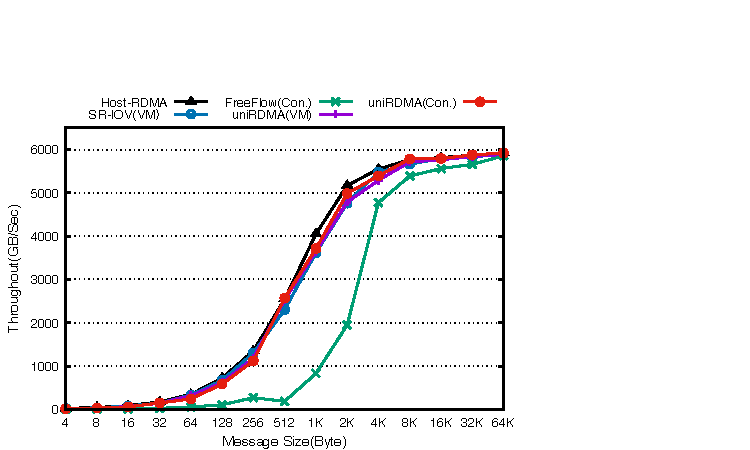
\includegraphics[width=1.0\linewidth]{images/send-bw.pdf}
	\caption{The Throughout of RDMA Send and Recv}
	\label{fig:send-bw}
\end{figure}

\begin{figure}[!ht]
	\centering
	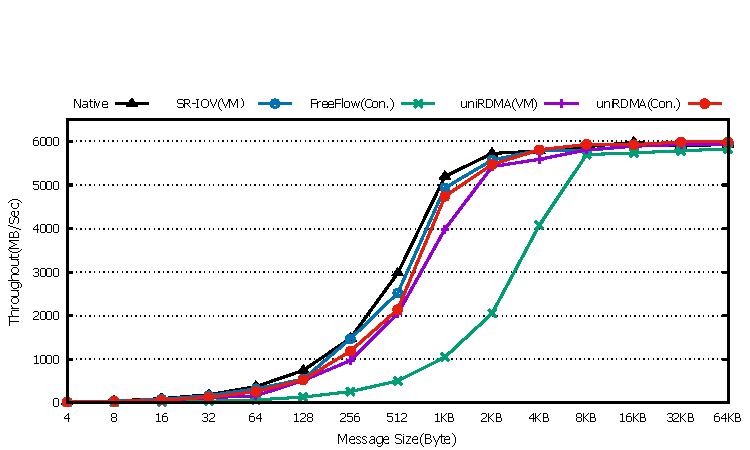
\includegraphics[width=1.0\linewidth]{images/write-bw.pdf}
	\caption{The Throughout of RDMA Write}
	\label{fig:write-bw}
\end{figure}

When the message gradually increases, such as reaching 64KB, the throughput of each framework tends to be consistent. The reason is that the bandwidth is saturated, and the delay overhead of FreeFlow has been covered by waiting delay in RNIC.

(2) Latency: The results of two-sided operation are shown in Figure~\ref{fig:send-lat}, and the one of one-sided operation are shown in Figure~\ref{fig:write-lat}. Whether \sys is in a virtual machine or in a container scenario, the latency of its two-sided and one-sided operations is similar as SR-IOV and close to native RDMA.

Compared with FreeFlow, when the message is small, the latency of \sys has reached 40\%~60\% of FreeFlow because of FreeFlow's forwarding latency. Also, when the message gradually increases, such as reaching 64KB, the latency of each framework tends to be consistent. Because the main latency has been caused by RNIC data processing.

\begin{figure}[!ht]
	\centering
	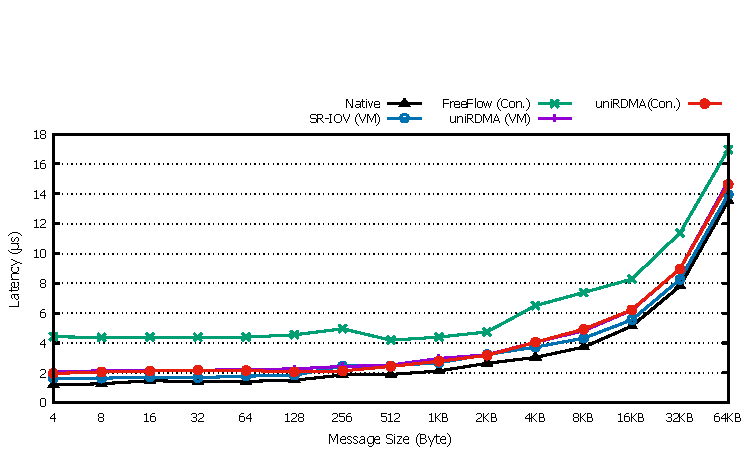
\includegraphics[width=1.0\linewidth]{images/send-lat.pdf}
	\caption{The Latency of RDMA Send and Recv}
	\label{fig:send-lat}
\end{figure}

\begin{figure}[!ht]
	\centering
	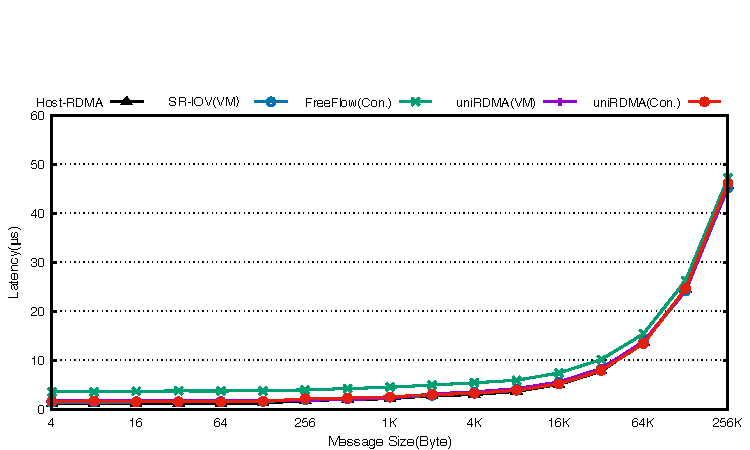
\includegraphics[width=1.0\linewidth]{images/write-lat.pdf}
	\caption{The Latencty of RDMA Write}
	\label{fig:write-lat}
\end{figure}

\subsection{Real-world Applications}

The worth of RDMA is mainly about its optimized performance in real-world applications. RDMA virtualization needs to maintain the performance close to native RDMA. Therefore, we evaluate \sys and other frameworks in high-performance computing benchmark Graph-500. Graph-500 is a benchmark framework used to test the performance of the Message Passing Interface (MPI). Based on the constructed graph structure, users test the performance of breadth-first search (BFS) and single source shortest path (SSSP). The performance index is the number of edges traversed per second (traversed edges). per second, TEPS), the larger the value, the better the performance.

In this paper, the node scale of the computational graph in Graph-500 is set to 26, and the ratio of edges to points is set to the default parameter of 16. The constructed graph has a total of 2$^{25}$ vertices, with 2$^{29}$ edges, the entire graph occupies approximately around 16GB. When testing BFS and SSP, 16 MPI processes are scattered and executed on two nodes in turn, and the average value is taken according to the results of 12 tests. The data obtained is shown in Table Figure~\ref{fig:graph-500} (because there are core dump problems when using FreeFlow for Graph-500, the corresponding data is lacking).

As shown in Figure~\ref{fig:graph-500},  the performance of \sys is close to native RDMA. Because \sys bypasses the kernel and virtualization layer in the data path, and there is no forwarding latency.

\begin{figure}[!ht]
	\centering
	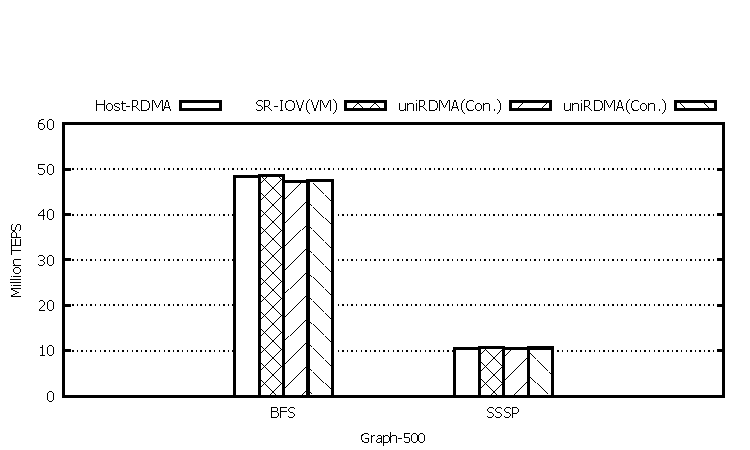
\includegraphics[width=1.0\linewidth]{images/graph-500.pdf}
	\caption{The Performance of Graph-500}
	\label{fig:graph-500}
\end{figure}
\section{Related Work} \label{relatedwork}

\textbf{Traditional TCP/IP:}\qquad TCP/IP is the basic network for each tenant in data centers. Several software solutions were proposed for traditional network virtualization. For both VMs and containers, virtual network interface cards (vRNICs) are one solution, e.g. virtio-net~\cite{virtio-russell2008}, vhost-net~\cite{vhost-net},  vhost-user-net~\cite{vhost-user-net} for VMs and veth~\cite{veth} for containers. These vRNICs are implemented in VM's or container's different space (i.e. kernel space and user space). Software-based switch, also knowed as virtual switch, in the local host brides the vNIC to physical NIC. Virtual switch can run in user space (e.g. Snabb Switch~\cite{snabb}), kernel space(e.g. Linux bridge~\cite{linux-bridge}), or both(e.g. Open vSwitch~\cite{ovs-2015}). 

\textbf{Hardware-based RDMA virtualization:}\qquad SR-IOV~\cite{sr-iov} splits a physical PCI-e device to multiple PCI-e devices, which can be allocated to VMs, providing near-native performance. In comparison to software-baed virtualization, it lacks of refficient resource management and suffers from the flexibility issue due to its virtual layer is realized in hardware. In uniRDMA, the isolation of SR-IOV are utilized and the unscalable problems are solved by dynamic vRNIC mapping. 

\textbf{Software-based RDMA virtualization:}\qquad FreeFlow~\cite{kim2019freeflow} forwards all RDMA commands from containers to the FreeFlow router (FFR) including data path. It intercepts the commands between applications and NIC drivers such as creating QP/CQ and sending/receiving data. The key different between FreeFlow and uniRDMA is that FreeFlow does capture data path commands to fitting in the container environment. Its data path commands, which accounts for the majority compared to the control path, costs extra forward latency. HyV~\cite{pfefferle2015hybrid} and MasQ~\cite{he2020masq} are designed for VMs. They achieve zero-copy and by-pass by mapping all resources. However, the implementation of memory mapping are different that is uniRDMA maps memory between virtual layer and VM's application. Moreover, HyV/MasQ backend is in kernel space while uniRDMA backend is in user space for more manageability and lightweight.

\section{Conclusion}
In this paper, we design a unified RDMA virtualization framework, namely uniRDMA, which consists of single user-space virtual layer and general uniVerbs interfaces. In the user space virtual layer: the isolated and high-performance vRNICs are virtualized based on the VFs from SR-IOV; In the uniVerbs interfaces: uniRDMA uses shared files to realize general I/O channel for VMs and containers; the isolation of interface is ensured with mount namespace in containers; uniVebrs realizes zero-copy and bypassing virtual layer in RDMA data path, by mapping all RDMA resource between vRNIC and RDMA applications. The experimental results show that uniRDMA has high performance close to native RDMA while meeting generality and management.


\bibliographystyle{ACM-Reference-Format}
\bibliography{reference}
\end{document}
\endinput
%%
%% End of file `sample-sigconf.tex'.
